\documentclass{article}
\usepackage{listings}
\usepackage{graphicx}
\usepackage{float}
\usepackage{fontspec}
\setsansfont{Ubuntu}% Ubuntu as sans - use \sffamily or \textsf{} as normal
\setmonofont{JetBrainsMono Nerd Font Mono}% Ubuntu Mono as 'typewriter' - use \ttfamily or \texttt{}
\usepackage[a4paper,
            bindingoffset=0.2in,
            left=1cm,
            right=1cm,
            top=1in,
            bottom=1in,
            footskip=.25in]{geometry}
\usepackage{hyperref}
\hypersetup{
    colorlinks, citecolor=black, filecolor=black,
    linkcolor=black, urlcolor=black
}
\usepackage{xcolor}
\definecolor{mygreen}{rgb}{0.05,0.15,0.11}
\definecolor{mygray}{rgb}{0.9,0.9,0.9}
\definecolor{mymauve}{rgb}{0.58,0,0.82}
\lstset{
  % backgroundcolor=\color{mygray}, 
  basicstyle=\ttfamily,
  breakatwhitespace=false,
  breaklines=true,
  % commentstyle=\color{darkgray},
  keepspaces=true,
  keywordstyle=\bfseries,
  morekeywords={*,...},
  showspaces=false,
  showstringspaces=false,
  showtabs=false,
  % stringstyle=\color{blue},
  tabsize=4,
  % numbers=left,
  rulecolor=\color{black},
  postbreak=\mbox{\textcolor{red}{$\hookrightarrow$}\space}
}

\begin{document}

\pagenumbering{gobble}
{\centerline{\bfseries \Huge Assignment 4}}

\section*{Question 1}
Write a JavaScript function to capitalize the first letter of each word in a string. \\
\textbf{Test Data :}
\begin{lstlisting}
  (capitalize_Words('js string exercises'));
  Output: "Js String Exercises"
\end{lstlisting}
\subsection*{Code}
\lstinputlisting[language=html]{1/index.html}
\newpage
\subsection*{Output}
\begin{figure}[H]
  \centering
  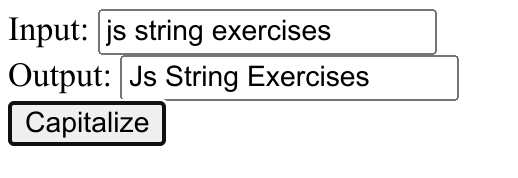
\includegraphics[width=10cm]{1/out.png}
\end{figure}

\newpage
\section*{Question 2}
Write a JavaScript function that takes a string which has lower and
upper case letters as a parameter and converts upper case letters to
lower case, and lower case letters to upper case. \\
\textbf{Test Data:}
\begin{lstlisting}
  (swapcase('AaBbc'));
  Output: "aAbBC"
\end{lstlisting}
\subsection*{Code}
\lstinputlisting[language=html]{2/index.html}
\newpage
\subsection*{Output}
\begin{figure}[H]
  \centering
  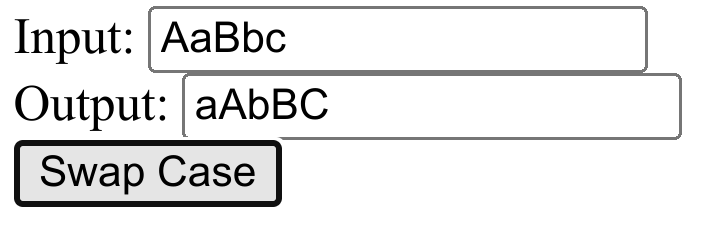
\includegraphics[width=10cm]{2/out.png}
\end{figure}

\newpage
\section*{Question 3}
Develop and demonstrate a HTML file that includes JavaScript script
that uses functions for the following problems:

\begin{itemize}
  \item Parameter: A string \\
  Output: The position in the string of the left-most vowel
  \item Parameter: A number \\
  Output: The number with its digits in the reverse order.
\end{itemize}
\subsection*{Code}
\lstinputlisting[language=html]{3/index.html}
\newpage
\subsection*{Output}
\begin{figure}[H]
  \centering
  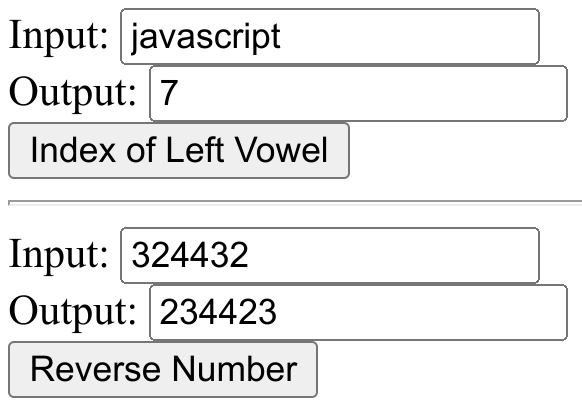
\includegraphics[width=10cm]{3/out.png}
\end{figure}

\newpage
\section*{Question 4}
Write a JavaScript function that takes a string as a parameter and
count occurrence of each alphabet in a given string.
\subsection*{Code}
\lstinputlisting[language=html]{4/index.html}
\newpage
\subsection*{Output}
\begin{figure}[H]
  \centering
  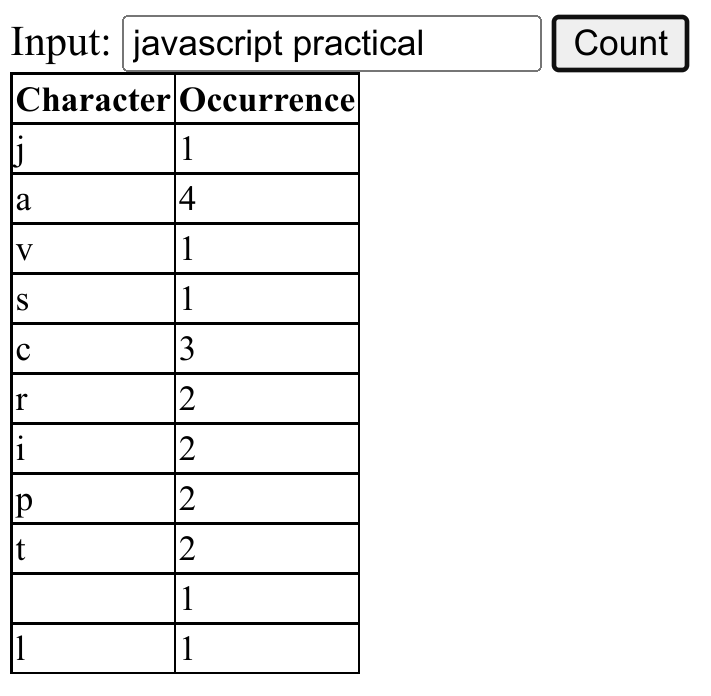
\includegraphics[width=10cm]{4/out.png}
\end{figure}
\end{document}